\chapter{Methodology}
\label{ch:method}

\section{The bond pullout test}
\label{sec:test}

The configuration modelled throughout this chapter is the concentric pull-out
test in its \emph{pull--push} form, the most widely used test for bond between a
deformed bar and concrete.

\noindent A single bar is cast centrally in a concrete prism or cylinder and protrudes from one face. The bar is gripped outside the specimen and loaded in direct
tension, while the concrete bears against a stiff reaction plate at the
\emph{same} face. The bar is therefore pulled and the concrete pushed, from which the configuration takes its name. The specimen is self-equilibrated: at every section the tensile force remaining in the bar is balanced by an equal compressive force in the surrounding concrete, and no external restraint acts on the far end.

The bonded length $L$ is not the full depth of the specimen. Plastic or PVC
sleeves are bonded to the bar over the remainder of its embedded length so
that bond develops only over a controlled zone, which allows $L$ to be varied
independently of specimen size. RC~6 specifies a bonded length of $5d_b$ with
the bond-free length placed adjacent to the loaded face, so that the bonded
zone lies outside the compression cone spreading from the reaction plate.
Instrumentation comprises a load cell in line with the bar and displacement
transducers measuring slip; free-end (unloaded-end) slip is normally preferred
to loaded-end slip because it excludes the elastic extension of the bar
between the grip and the specimen face.

Two consequences of this arrangement matter for the interpretation of the
model and of the comparisons in Chapter~[X].

The bearing reaction places the concrete surrounding the bonded length in
\emph{axial compression}, and the resulting transverse confinement suppresses
splitting. Pull-out tests therefore return higher bond strengths, and are more
likely to produce a pull-out rather than a splitting failure, than
arrangements in which the concrete is in tension---a lapped splice, a beam-end
test, or the pull--pull configuration treated by
\textcite{alaviAnalyticalProcedureFailure2025}. Capacities derived from
pull-out data are consequently an upper bound on what is available in a
tension member, and the model inherits that bias.

The short bonded length prescribed by RC~6 is chosen deliberately so that the
bond stress is approximately \emph{uniform} over the bonded zone, allowing the
measured capacity to be reported as a single average bond strength
$\tau_u = F_u/(\pi d_b L)$. The present model makes no such assumption: it
resolves the full distribution of bond stress along $z$, and
Section~\ref{sec:calibration} shows that the distribution is strongly
non-uniform once $L$ exceeds a few diameters. The two are consistent at short
bonded lengths and diverge as $L$ grows, which is the central reason for
sweeping $L/d_b$ rather than working at a single standardised length.

\begin{figure}[htbp]
  \centering
   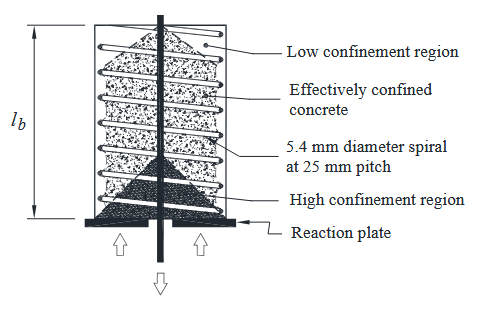
\includegraphics[width=0.7\textwidth]{test setup.png}
  \caption{Bond pullout test specimen: bar, bonded length
           $L$, reaction plate and clearance hole.}
  \label{fig:pullout}
\end{figure}

\subsection{Idealisation of the specimen}
\label{sec:idealisation}

The model represents this specimen as follows. A cubic or prismatic specimen
is replaced by an equivalent concentric cylinder of outer radius $r_e$, chosen
to preserve the concrete cross-sectional area or the minimum cover, whichever
the comparison requires; a cylinder of \SI{150}{\milli\metre} diameter is used
here. The debonded zones carry no shear and are therefore outside the domain:
the model's $z = 0$ is the start of the bonded length and $z = L$ its end, not
the specimen faces. The reaction plate enters only as the boundary condition
$\sigma_z^{c}(0) = -q$ of Eq.~\eqref{eq:bcaxial}, which transmits the full bar
force into the concrete in bearing at the loaded end of the bonded zone.

This last point is an approximation worth stating plainly. In the standard
specimen the bond-free length separates the bonded zone from the plate, so the
bearing stress has partly dispersed before it reaches $z = 0$; in the model
the two are coincident. The idealisation is therefore slightly conservative
with respect to the hoop stress at the loaded end, where the dispersal would
relieve some of the splitting demand.

\section{Three-layer model and assumptions}
\label{sec:scope}

The model predicts the elastic stress field in a single deformed bar bonded in a concrete cylinder, and from it the governing failure mode, the load-carrying capacity, the elastic bond stiffness and the slip at failure.
It follows the variational procedure introduced by
\textcite{nemesModelingCylindricalAdhesively2009} for cylindrical adhesively
bonded joints and extended by \textcite{alaviAnalyticalProcedureFailure2025}
to glued-in rod (GiR) timber connections, with the timber adherend replaced by
concrete and the adhesive layer reinterpreted as a thin \emph{rib layer}
representing the mechanically interlocked annulus immediately surrounding the
bar.

\noindent The specimen is idealised as three concentric, axisymmetric, linearly elastic
cylinders over the embedded length $L$:

\begin{table}[htbp]
\centering
\begin{tabular}{lll}
\hline
Zone & Radial extent & Properties \\
\hline
Bar       & $r_i < r < r_s$ & $E_s,\ \nu_s,\ G_s$ \\
Rib layer & $r_s < r < r_r$ & $E_r,\ \nu_r,\ G_r$ \\
Concrete  & $r_r < r < r_e$ & $E_c,\ \nu_c,\ G_c$ \\
\hline
\end{tabular}
\caption{Zones of the three-layer idealisation.}
\label{tab:zones}
\end{table}

\noindent with $r_i = 0$ for a solid bar. All three materials are taken as
isotropic, $G = E/[2(1+\nu)]$. The rib layer is presently assigned the concrete
properties, so its role is geometric---it carries the discontinuity in shear
and hoop stress between bar and concrete---and it provides the single
parameter, $t_{\mathrm{rib}} = r_r - r_s$, through which rib geometry can
later be introduced.

\noindent The analysis adopts the hypotheses of
\textcite{nemesModelingCylindricalAdhesively2009}: axisymmetry suppresses
$\tau_{r\theta}$ and $\tau_{z\theta}$; the axial stress in the rib layer is
neglected, $\sigma_z^{r} = 0$; the axial stresses in the bar and the concrete
are functions of $z$ alone; and the radial stresses vary with $r$ alone. The
entire field is expressed in terms of one unknown function, the bar axial
stress $\sigma(z) \equiv \sigma_z^{s}(z)$, and one unknown scalar, the
radial-stress parameter $\alpha_1$.

\noindent With $A_s = \pi(r_s^2 - r_i^2)$ and $A_c = \pi(r_e^2 - r_r^2)$, an applied load
$F$ produces a bar stress $f = F/A_s$ at the loaded end and a nominal bearing
stress $q = F/A_c$ on the concrete face.

\section{Assumed stress field}
\label{sec:field}

Axial and radial equilibrium of an axisymmetric element,
\begin{equation}
\label{eq:equilibrium}
\frac{\partial}{\partial r}\!\left[r\sigma_r^{(i)}\right]
  + \frac{\partial}{\partial z}\!\left[r\tau_{rz}^{(i)}\right]
  = \sigma_\theta^{(i)},
\qquad
\frac{\partial}{\partial r}\!\left[r\tau_{rz}^{(i)}\right]
  + \frac{\partial}{\partial z}\!\left[r\sigma_z^{(i)}\right] = 0,
\end{equation}
following Eqs.~(6)--(7) of \textcite{nemesModelingCylindricalAdhesively2009}. The radial
stresses are assumed to vary \emph{linearly} and to vanish on the two free
surfaces, $r = r_i$ and $r = r_e$, after Eq.~(8) of
\textcite{nemesModelingCylindricalAdhesively2009}:
\begin{equation}
\label{eq:radial}
\sigma_r^{s} = \alpha_1 (r - r_i), \qquad
\sigma_r^{r} = \text{const.}, \qquad
\sigma_r^{c} = \alpha_2 (r - r_e).
\end{equation}

Continuity of $\sigma_r$ across both interfaces---a consequence of momentum
conservation at a closed interface, as noted in Eq.~(13) of
\textcite{alaviAnalyticalProcedureFailure2025}---fixes the rib-layer constant
and $\alpha_2$:
\begin{equation}
\label{eq:continuity}
\sigma_r^{r} = \alpha_1 (r_s - r_i), \qquad
\alpha_2 = \frac{\alpha_1 (r_s - r_i)}{r_r - r_e}.
\end{equation}

The linear form \eqref{eq:radial} is Nemes and Lachaud's;
\textcite{alaviAnalyticalProcedureFailure2025} replace it with a quadratic
variation, $\sigma_r^{s} = \Lambda_1 r^2$ and
$\sigma_r^{t} = \Lambda_3(r^2 - r_t^2)$ (their Eq.~6), which they show
improves agreement with FE near the loaded end. The linear form is retained
here because it leaves a single unknown $\alpha_1$ and keeps every radial
integral elementary; the quadratic refinement is identified in Section~[X] as
the first candidate improvement.

Integrating \eqref{eq:equilibrium} subject to
\eqref{eq:radial}--\eqref{eq:continuity} and to continuity of $\tau_{rz}$ at
both interfaces gives the complete field in terms of $\sigma(z)$, reproducing
Eqs.~(12)--(13), (15)--(16) and (19)--(20) of
\textcite{nemesModelingCylindricalAdhesively2009}.

\paragraph{Bar, $r_i < r < r_s$.}
\begin{equation}
\label{eq:bar}
\sigma_z^{s} = \sigma, \qquad
\tau_{rz}^{s} = \frac{r_i^2 - r^2}{2r}\,\sigma', \qquad
\sigma_\theta^{s} = \frac{r_i^2 - r^2}{2}\,\sigma'' + \alpha_1(2r - r_i).
\end{equation}

\paragraph{Rib layer, $r_s < r < r_r$.}
\begin{equation}
\label{eq:rib}
\sigma_z^{r} = 0, \qquad
\tau_{rz}^{r} = \frac{r_i^2 - r_s^2}{2r}\,\sigma', \qquad
\sigma_\theta^{r} = \alpha_1(r_s - r_i) + \frac{r_i^2 - r_s^2}{2}\,\sigma''.
\end{equation}

\paragraph{Concrete, $r_r < r < r_e$.}
\begin{equation}
\label{eq:conc}
\tau_{rz}^{c} = \frac{(r_e^2 - r^2)(r_i^2 - r_s^2)}{2r\,(r_e^2 - r_r^2)}\,\sigma',
\qquad
\sigma_\theta^{c} = \frac{(r_i^2 - r_s^2)(r_e^2 - r^2)}{2(r_e^2 - r_r^2)}\,\sigma''
                    + \alpha_2(2r - r_e).
\end{equation}

The concrete axial stress follows from assembly equilibrium, the rib layer
carrying no axial load. For the self-equilibrated pull--push specimen the bar
force is reacted entirely by the concrete at every section, so (cf.\ Eq.~(11b)
of \textcite{alaviAnalyticalProcedureFailure2025})
\begin{equation}
\label{eq:szc}
\sigma_z^{c} = -\,\frac{(r_s^2 - r_i^2)\,\sigma}{r_e^2 - r_r^2}
             = -\frac{A_s}{A_c}\,\sigma .
\end{equation}

Two structural features of \eqref{eq:bar}--\eqref{eq:szc} are used repeatedly
below. The shear stress is proportional to $\sigma'$ and the hoop stress to
$\sigma''$ plus a term linear in $\alpha_1$, so both separate into a function
of $r$ times a function of $z$; and every component is linear in the applied
load, which is what makes the capacity scaling of Section~\ref{sec:failure}
and the sweep of Section~\ref{sec:calibration} possible.

Continuity of $\sigma_r$ and $\tau_{rz}$ at $r = r_s$ and $r = r_r$ is
verified symbolically before the energy integration, as a check on
\eqref{eq:radial}--\eqref{eq:szc}.

\section{Strain energy}
\label{sec:energy}
 
The strain energy of each layer is obtained by integrating the complementary
energy density over its annulus and along the bonded length, after Eq.~(21) of
\textcite{nemesModelingCylindricalAdhesively2009} and Eq.~(17) of
\textcite{alaviAnalyticalProcedureFailure2025}:
\begin{align}
\label{eq:energy-steel}
U^{s} &= \pi \int_0^L \!\! \int_{r_i}^{r_s}
  \left[ \frac{\sigma_\theta^{s2}}{E_s}
       + \frac{\sigma_z^{s2}}{E_s}
       - \frac{2\nu_s}{E_s}\,\sigma_z^{s}\sigma_\theta^{s}
       + \frac{\tau_{rz}^{s2}}{G_s} \right] r\,\mathrm{d}r\,\mathrm{d}z , \\[8pt]
\label{eq:energy-rib}
U^{r} &= \pi \int_0^L \!\! \int_{r_s}^{r_r}
  \left[ \frac{\sigma_\theta^{r2}}{E_r}
       + \frac{\tau_{rz}^{r2}}{G_r} \right] r\,\mathrm{d}r\,\mathrm{d}z , \\[8pt]
\label{eq:energy-conc}
U^{c} &= \pi \int_0^L \!\! \int_{r_r}^{r_e}
  \left[ \frac{\sigma_\theta^{c2}}{E_c}
       + \frac{\sigma_z^{c2}}{E_c}
       - \frac{2\nu_c}{E_c}\,\sigma_z^{c}\sigma_\theta^{c}
       + \frac{\tau_{rz}^{c2}}{G_c} \right] r\,\mathrm{d}r\,\mathrm{d}z ,
\end{align}
and the total strain energy of the assembly is
\begin{equation}
\label{eq:energy}
U = U^{s} + U^{r} + U^{c} .
\end{equation}
 
Substituting the assumed field \eqref{eq:bar}--\eqref{eq:szc} into
\eqref{eq:energy-steel}--\eqref{eq:energy-conc} makes it possible to write the
strain energy in terms of $\sigma_z^{s}$ and its derivatives alone, as in
Eq.~(22) of \textcite{nemesModelingCylindricalAdhesively2009}:
\begin{equation}
\label{eq:quadform}
U = \pi \int_0^L \Gamma \,\mathrm{d}z ,
\end{equation}
in which the integrand is
\begin{equation}
\label{eq:gamma}
\begin{split}
\Gamma = {}& A\,\sigma_z^{s2}
   + B\,\sigma_z^{s}\,\frac{\mathrm{d}^2\sigma_z^{s}}{\mathrm{d}z^2}
   + C\left(\frac{\mathrm{d}\sigma_z^{s}}{\mathrm{d}z}\right)^{\!2}
   + \tilde{D}\,\sigma_z^{s} \\[8pt]
 &{} + E\left(\frac{\mathrm{d}^2\sigma_z^{s}}{\mathrm{d}z^2}\right)^{\!2}
   + \tilde{F}\,\frac{\mathrm{d}^2\sigma_z^{s}}{\mathrm{d}z^2}
   + \tilde{K} ,
\end{split}
\end{equation}
and
\begin{equation}
\label{eq:coeffs}
\tilde{D} = D + \alpha_1 k, \qquad
\tilde{F} = F + \alpha_1 h, \qquad
\tilde{K} = K + \alpha_1^2 m .
\end{equation}
 
The coefficients $A$--$K$ and $h$, $k$, $m$ are functions of the radii and the
elastic constants only, and carry no dependence on $z$ or on the applied load.
They are obtained by expanding the energy density and taking partial
derivatives with respect to $\sigma_z^{s}$ and its derivatives, evaluated at
zero. 

Their closed forms are lengthy, involving the logarithms $\ln(r_r/r_s)$ and $\ln(r_e/r_r)$ returned
by the integrals, and are set out in full in Appendix~[X]. The absence
of a term linear in $\alpha_1$ in $\tilde{K}$ is specific to the pull--push
configuration, where \eqref{eq:szc} contains no constant contribution from the
applied load.

\newpage
\section{Governing differential equation and its solution}
\label{sec:ode}

Requiring the strain energy to be stationary, $\delta U = 0$, and
applying the Euler--Lagrange equation of the functional \eqref{eq:quadform}
gives the governing equation, Eq.~(26) of
\textcite{nemesModelingCylindricalAdhesively2009}:
\begin{equation}
\label{eq:ode}
E\,\frac{\mathrm{d}^4\sigma_z^{s}}{\mathrm{d}z^4}
  + (B - C)\,\frac{\mathrm{d}^2\sigma_z^{s}}{\mathrm{d}z^2}
  + A\,\sigma_z^{s} + \frac{\tilde{D}}{2} = 0 .
\end{equation}

This is a linear, fourth-order, constant-coefficient ordinary differential
equation and is solved in closed form. Its characteristic roots are
\begin{equation}
\label{eq:roots}
\lambda_{1,2}^2 = \frac{-(B - C) \pm \sqrt{(B - C)^2 - 4AE}}{2E},
\end{equation}
equivalent to $\varpi_{1,2}$ in Eq.~(21) of
\textcite{alaviAnalyticalProcedureFailure2025}, and the general solution is
\begin{equation}
\label{eq:solution}
\sigma_z^{s}(z) = C_1 e^{\lambda_1 z} + C_2 e^{-\lambda_1 z}
          + C_3 e^{\lambda_2 z} + C_4 e^{-\lambda_2 z}
          - \frac{\tilde{D}}{2A} .
\end{equation}

No numerical integration, discretisation or shooting is used at any stage; the
solution is analytical throughout, and the only numerical operations are the
evaluation of \eqref{eq:solution} and the stress averaging of
Section~\ref{sec:failure}.

\section{Boundary conditions and the radial-stress parameter}
\label{sec:closure}

\subsection{Boundary conditions}
\label{sec:bc}

Four conditions determine $C_1 \dots C_4$. The bonded length terminates at
free surfaces, so the interface shear vanishes there,
\begin{equation}
\label{eq:bcshear}
\tau_{rz}^{s}(z = 0) = \tau_{rz}^{s}(z = L) = 0 ,
\end{equation}

The two axial conditions express the pull--push arrangement through
\eqref{eq:szc}: the concrete carries the full bearing stress at the loaded
face and is unstressed at the free end,
\begin{equation}
\label{eq:bcaxial}
\sigma_z^{c}(0) = -q, \qquad \sigma_z^{c}(L) = 0,
\end{equation}
equivalently $\sigma_z^{s}(0) = f$ and $\sigma_z^{s}(L) = 0$, i.e.\ complete transfer of
the bar force to the concrete over the embedded length. These are the
pull--push conditions of Eq.~(22b) of
\textcite{alaviAnalyticalProcedureFailure2025}. The four conditions are
assembled into a linear system and solved symbolically, so $C_1 \dots C_4$ are
obtained as explicit functions of the geometry, the moduli, the load and
$\alpha_1$.

\subsection{Determination of \texorpdfstring{$\alpha_1$}{alpha 1}}
\label{sec:alpha}
 
\begingroup
% A little more air around the displays in this subsection, and no shrink, so
% the equations are spaced evenly rather than squeezed to fill the page.
\setlength{\abovedisplayskip}{13pt plus 3pt minus 1pt}
\setlength{\belowdisplayskip}{13pt plus 3pt minus 1pt}
\setlength{\abovedisplayshortskip}{8pt plus 2pt minus 1pt}
\setlength{\belowdisplayshortskip}{8pt plus 2pt minus 1pt}
 
$\alpha_1$ is the one remaining unknown and is fixed by making the energy
stationary with respect to it, $\partial U/\partial\alpha_1 = 0$. Since
$\alpha_1$ enters $\Gamma$ only through $\tilde{D}$, $\tilde{F}$ and
$\tilde{K}$, differentiating \eqref{eq:quadform}--\eqref{eq:coeffs} gives
\begin{equation}
\label{eq:alphastat}
2m\alpha_1 L + \int_0^L \left( k\,\sigma_z^{s}
  + h\,\frac{\mathrm{d}^2\sigma_z^{s}}{\mathrm{d}z^2} \right)\,\mathrm{d}z = 0 ,
\end{equation}
in which the second term integrates to
$h\left[\mathrm{d}\sigma_z^{s}/\mathrm{d}z\right]_0^L$ and vanishes
identically by the boundary condition \eqref{eq:bcshear}, leaving
\begin{equation}
\label{eq:alphared}
2m\alpha_1 L + \int_0^L k\,\sigma_z^{s}\,\mathrm{d}z = 0 .
\end{equation}
 
Equation~\eqref{eq:alphared} is implicit in appearance, since $\sigma_z^{s}$
was itself constructed from $\alpha_1$, but the dependence is affine in both
places it arises---the particular solution $-(D + \alpha_1 k)/2A$, and the
constants $C_1 \dots C_4$, whose linear system carries that particular
solution on its right-hand side. The field therefore splits exactly into its
$\alpha_1$-independent and $\alpha_1$-linear parts,
\begin{equation}
\label{eq:affine}
\sigma_z^{s}(z) = \sigma_0(z) + \alpha_1\,\sigma_1(z),
\qquad
\sigma_0 = \left.\sigma_z^{s}\right|_{\alpha_1 = 0},
\qquad
\sigma_1 = \frac{\partial \sigma_z^{s}}{\partial \alpha_1},
\end{equation}
both functions of $z$ alone. Substituting \eqref{eq:affine} into
\eqref{eq:alphared} and using the linearity of the integral,
\begin{equation}
\label{eq:alphaexpand}
2m\alpha_1 L + \int_0^L k\,\sigma_0(z)\,\mathrm{d}z
  + \alpha_1 \int_0^L k\,\sigma_1(z)\,\mathrm{d}z = 0 ,
\end{equation}
with $\alpha_1$ taken outside the second integral because $\sigma_1$ does not
depend on it. The two definite integrals are
\begin{equation}
\label{eq:I0I1}
I_0 = k \int_0^L \left.\sigma_z^{s}\right|_{\alpha_1 = 0}\,\mathrm{d}z ,
\qquad
I_1 = k \int_0^L \frac{\partial \sigma_z^{s}}{\partial \alpha_1}\,\mathrm{d}z ,
\end{equation}
where $k$ comes outside because it depends only on the radii and the elastic
constants. Neither integral contains $\alpha_1$, so \eqref{eq:alphaexpand} is
one linear equation in the one unknown and closes the problem exactly,
without iteration:
\begin{equation}
\label{eq:alpha}
2m\alpha_1 L + I_0 + \alpha_1 I_1 = 0
\qquad\Longrightarrow\qquad
\alpha_1 = -\,\frac{I_0}{2mL + I_1} .
\end{equation}
 
Substituting \eqref{eq:alpha} into \eqref{eq:solution} and then into
\eqref{eq:bar}--\eqref{eq:szc} yields the complete stress field. All symbolic
manipulation uses exact rational arithmetic, and material values are
substituted only at this stage at 50 significant digits: the boundary-value
system is built on $e^{\pm\lambda z}$, whose two branches differ in magnitude
by $e^{2\lambda L}$ across the bonded length, so its condition number grows
exponentially with $\lambda L$ and double precision is exhausted well before
the longest case in the sweep.
\par
\endgroup

\section{Bond Stiffness}
\label{sec:stiffness}
 
\begingroup
\setlength{\abovedisplayskip}{13pt plus 3pt minus 1pt}
\setlength{\belowdisplayskip}{13pt plus 3pt minus 1pt}
\setlength{\abovedisplayshortskip}{8pt plus 2pt minus 1pt}
\setlength{\belowdisplayshortskip}{8pt plus 2pt minus 1pt}
 
The stress field of Section~\ref{sec:closure} also fixes the stiffness of the
anchorage, which governs behaviour at service load as the criteria of
Section~\ref{sec:failure} govern it at ultimate. Following Section~3 of
\textcite{alaviAnalyticalProcedureFailure2025}, the displacement of the loaded
end is recovered from the strain energy rather than by integrating the strain
field. Loading is monotonic and the assembly linearly elastic, so the external
work done by the applied load $F$ as it is brought up from zero equals the
strain energy stored,
\begin{equation}
\label{eq:work}
U = \frac{F\,\delta}{2} ,
\end{equation}
whence the axial displacement of the loaded end is
\begin{equation}
\label{eq:slip}
\delta = \frac{2U}{F} ,
\qquad
U = \pi \int_0^L \Gamma \,\mathrm{d}z ,
\end{equation}
with $\Gamma$ from \eqref{eq:gamma} evaluated on the closed-form solution
\eqref{eq:solution}. The integrand is a quadratic form in sums of
exponentials, so $U$ follows from the same elementary integrals as
\eqref{eq:I0I1} and no quadrature is required. 
The bond stiffness is
the ratio of load to displacement, 
\begin{equation}
\label{eq:kbond}
k_s = \frac{F}{\delta} = \frac{F^2}{2U} .
\end{equation}
 
Equation~\eqref{eq:kbond} does not depend on the applied load. The energy
coefficients $D$, $F$ and $K$ of \eqref{eq:coeffs} all vanish for the
pull--push configuration, so $\Gamma$ is a homogeneous quadratic form in
$\sigma_z^{s}$, its derivatives and $\alpha_1$, every one of which is
proportional to the load. Hence, $U$ scales as the square of the load, the
ratio $F^2/2U$ is unchanged by it, and $k_s$ is a property of the geometry and
the moduli alone, computed once per case alongside the capacity. The
displacement at failure follows directly,
\begin{equation}
\label{eq:slipfail}
\delta_u = \frac{F_u}{k_s} ,
\end{equation}
with $F_u$ from \eqref{eq:capacity}.
 
Two limitations bear on the comparison with test data in Chapter~[X]. First,
$\delta$ is the displacement of the loaded end relative to the bearing face
and includes the elastic extension of the bar and the compression of the
concrete; it is neither the relative slip across the interface nor the
free-end slip usually reported in pull-out tests, and is comparable only with
a measured loaded-end displacement. Second, the model is linearly elastic with
no bond degradation or interface softening represented, so $k_s$ is the
\emph{initial} stiffness and \eqref{eq:slipfail} extrapolates it linearly to
the failure load. Since a measured bond--slip curve softens progressively, the
predicted slip at failure is a lower bound on the measured value and $k_s$ an
upper bound on the secant stiffness at peak load; the comparison in
Chapter~[X] is accordingly made against the initial branch of the measured
response wherever the test data permit it.
\par
\endgroup

\section{Failure criteria}
\label{sec:failure}

Two failure modes are considered, both adapted from the six-mode framework of
\textcite{alaviAnalyticalProcedureFailure2025}; modes III--VI of that work are
specific to the anisotropy of timber and have no concrete counterpart.

\subsection{Mode I: yielding of the bar}
\label{sec:modeI}

Adapting Eq.~(27a) of \textcite{alaviAnalyticalProcedureFailure2025}, with the
peak bar stress occurring at the loaded end where $\sigma = f$,
\begin{equation}
\label{eq:modeI}
\varphi_{\mathrm{I}} = \frac{\sigma_z^{s}}{f_{sy}} - 1,
\qquad F_{\mathrm{I}} = f_{sy} A_s .
\end{equation}

\subsection{Mode II: cracking of the concrete}
\label{sec:modeII}
 
The quadratic interaction of Eq.~(28) of
\textcite{alaviAnalyticalProcedureFailure2025}, there written for the
adhesive, is applied to the hoop and shear stresses in the rib layer and the
surrounding concrete:
\begin{equation}
\label{eq:modeII}
\varphi_{\mathrm{II}} =
  \left(\frac{\bar{\sigma}_\theta}{f_t}\right)^{2}
+ \left(\frac{\bar{\tau}_{rz}}{f_v}\right)^{2} - 1,
\qquad f_t = f_v = 0.5\sqrt{f'_c} .
\end{equation}
Only tensile hoop stress drives splitting, so $\bar{\sigma}_\theta$ is
replaced by $\max(\bar{\sigma}_\theta, 0)$; compressive hoop makes no
contribution. Failure in either mode corresponds to $\varphi = 0$.
 
The strength $f_t$ is the \emph{mean} uniaxial tensile strength of the
concrete. AS~3600 gives the lower characteristic uniaxial tensile strength as
$f'_{ct} = 0.36\sqrt{f'_c}$, with the mean and upper characteristic values
obtained by multiplying it by $1.4$ and $1.8$ respectively
\parencite{ReinforcedConcreteBasics2021}, so that
\begin{equation}
\label{eq:ft}
f_t = 1.4 \times 0.36\sqrt{f'_c} = 0.5\sqrt{f'_c} .
\end{equation}
The mean rather than the characteristic value is appropriate here because the
model is compared against the measured capacities of individual specimens
rather than used in design: since both strengths in \eqref{eq:modeII} are
squared, adopting the lower characteristic value would reduce every predicted
capacity by exactly the factor $1.4$. Setting $f_v = f_t$ is a
simplification, made because no independent shear strength is available for
plain concrete and because failure under the combined state of
\eqref{eq:modeII} is in any case a tensile separation mechanism; a distinct
$f_v$ could be introduced without altering the formulation.

\newpage
\subsection{The theory of critical distances}
\label{sec:tcd}

Applying \eqref{eq:modeII} pointwise to an elastic field predicts cracking as
soon as the peak stress touches the strength, which grossly underestimates
brittle capacity because the stress concentration at the loaded end is both
severe and highly localised.
\textcite{alaviAnalyticalProcedureFailure2025} address the same difficulty by
averaging $\sigma_{\theta\theta}$ and $\tau_{rz}$ over a fracture length of
\SI{20}{\milli\metre}. Here the generalisation of that device due to
\textcite{taylorGeometricalEffectsFatigue1999,taylorTheoryCriticalDistances2010}
is adopted. The Theory of Critical Distances unifies several non-local
criteria distinguished only by the geometry over which the elastic field is
averaged: the Point Method samples at a single location $l_{\mathrm{ch}}/2$
ahead of the stress raiser, the Line Method averages along a line of length
$2\,l_{\mathrm{ch}}$, and the Area Method averages over a semicircle of radius
$1.32\,l_{\mathrm{ch}}$ \parencite{taylorTheoryCriticalDistances2010}. The
Area Method is adopted here because it samples the field in both the axial and
radial directions and is therefore the least sensitive to the strongly
biaxial character of the stress state at the bar surface. The stresses
entering \eqref{eq:modeII} are accordingly the means over a semicircular area
of radius
\begin{equation}
\label{eq:Ravg}
R = 1.32\,l_{\mathrm{ch}},
\end{equation}
centred on the point being assessed, where the coefficient $1.32$ is Taylor's
calibration of the semicircular averaging area against the Point and Line
Methods for a sharp crack
\parencite{taylorGeometricalEffectsFatigue1999,taylorTheoryCriticalDistances2010},
and $l_{\mathrm{ch}}$ is the critical distance, taken as
\SI{20}{\milli\metre} after
\textcite{alaviAnalyticalProcedureFailure2025}. The semicircle lies in the
$(z, r)$ plane and sits on the bar surface, since no material exists below
$r = r_s$.

\begin{figure}[H]
  \centering
  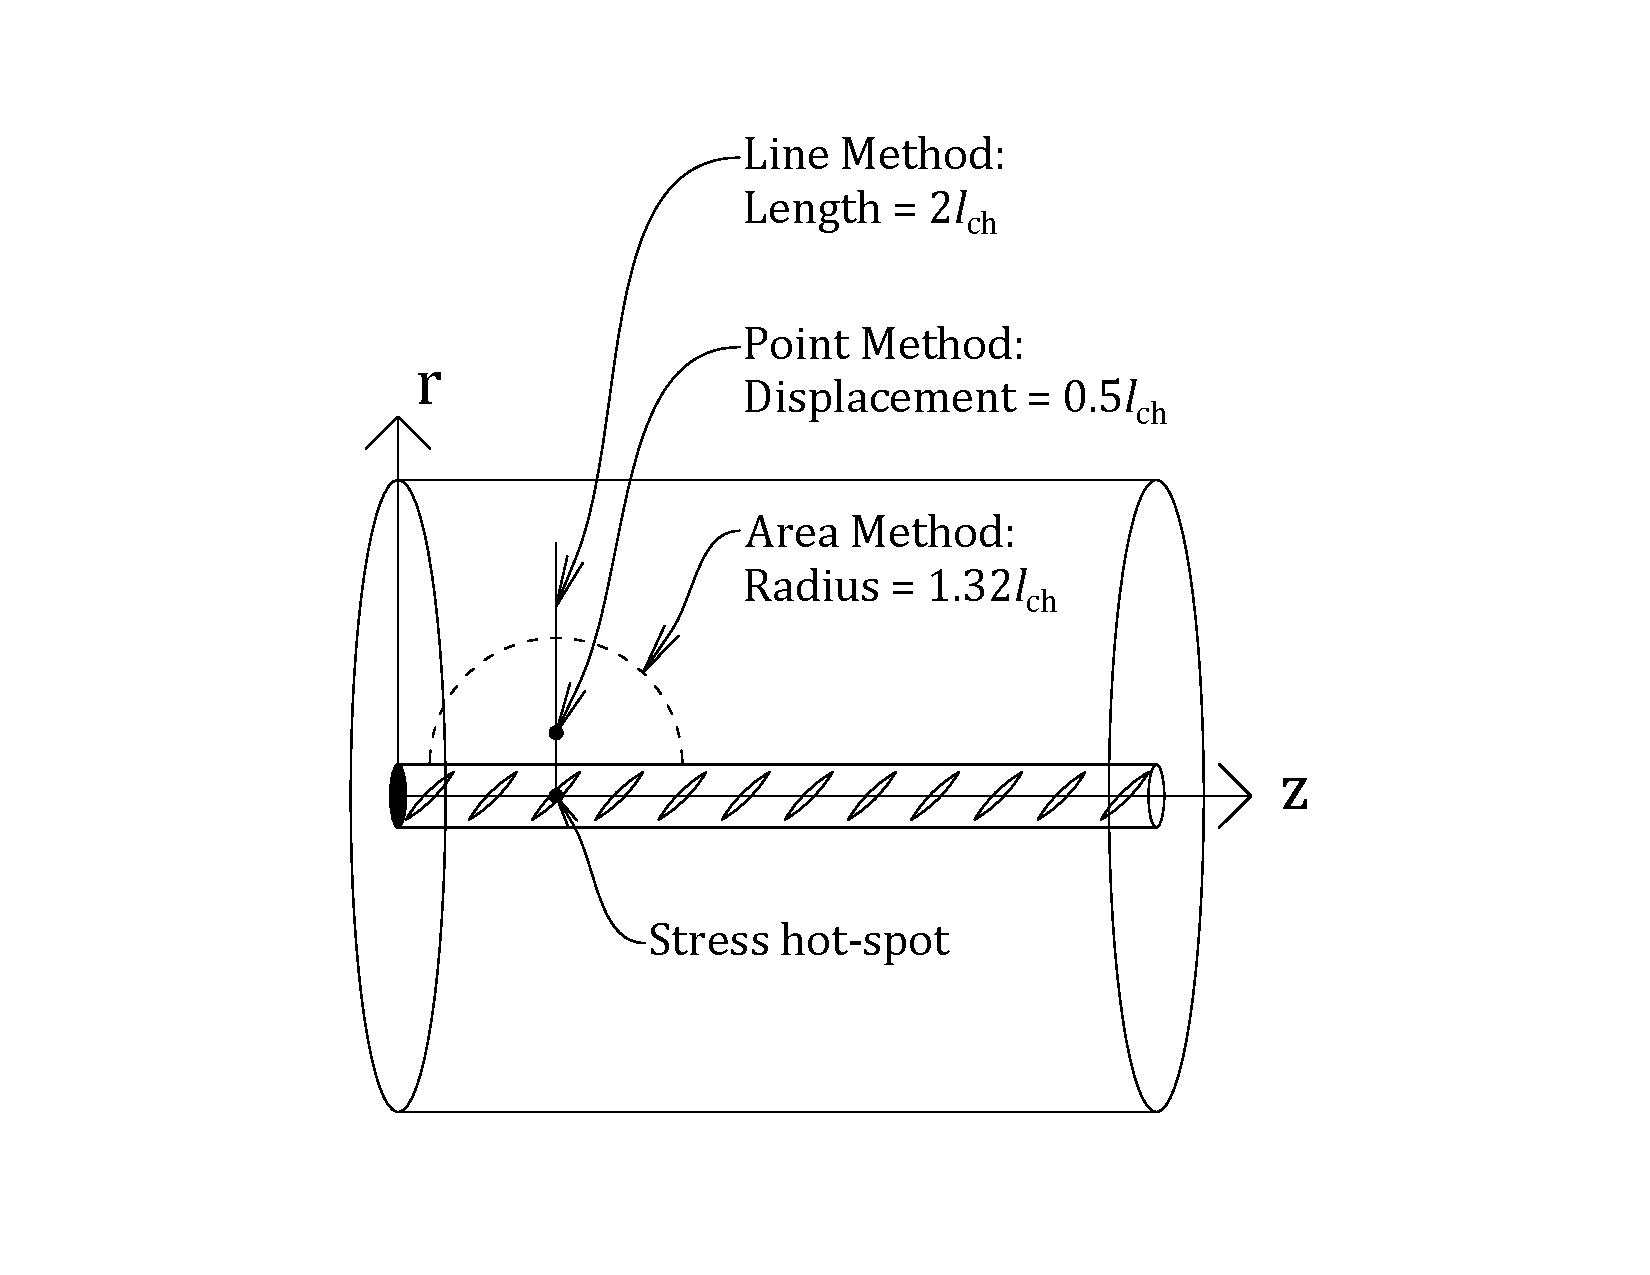
\includegraphics[width=0.55\textwidth]{critical_distances_1}
  \caption[The three Theory of Critical Distances averaging
           geometries]{The three averaging methods of the Theory of
           Critical Distances, shown at a stress hot-spot on the bar surface
           in the $(z, r)$ plane.}
  \label{fig:tcd}
\end{figure}
\newpage
The procedure is summarised in Figure~\ref{fig:areamethod}.
 
\begin{figure}[H]
\centering
\begin{tikzpicture}[
  node distance = 5.5mm,
  font = \small,
  term/.style = {rectangle, draw, rounded corners=7pt, align=center,
                 text width=80mm, inner sep=5pt},
  box/.style  = {rectangle, draw, align=left,
                 text width=80mm, inner sep=5pt},
  dec/.style  = {diamond, draw, aspect=2.8, align=center, inner sep=0pt,
                 text width=22mm, font=\footnotesize},
  arr/.style  = {-{Latex[length=2mm]}, thick}
]
 
\node[box] (p1)
  {\textbf{1\, Set the averaging size.}\\
   Critical distance $l_{\mathrm{ch}}$, item side $l_{\mathrm{item}}$,
   averaging radius $R = 1.32\,l_{\mathrm{ch}}$};
 
\node[box, below=of p1] (p2)
  {\textbf{2\, Lay out the item grid.}\\
   Divide the $(z,r)$ plane into squares of side $l_{\mathrm{item}}$ and
   compute $\tau_{rz}$ and $\sigma_\theta$ at the centre of each one};
 
\node[box, below=of p2] (p3)
  {\textbf{3\, Build the stencil, once.}\\
   Keep every square whose \emph{centre} lies within $R$ of the point being
   assessed. The half-disc reaches outward in $r$ from the bar surface and
   along $z$ in both directions};
 
\node[box, below=of p3] (p4)
  {\textbf{4\, Place the half-disc at station $z_0$.}\\
   Discard any square falling outside the bonded length, $z<0$ or $z>L$, so
   the disc is clipped near the two ends};
 
\node[box, below=of p4] (p5)
  {\textbf{5\, Average over the squares that remain.}\\
   $\bar\tau_{rz}(z_0)$ and $\bar\sigma_\theta(z_0)$, taken over the
   \emph{same} squares so the two are co-located};
 
\node[box, below=of p5] (p6)
  {\textbf{6\, Evaluate the Mode~II index at $z_0$.}\\
   $\varphi_{\mathrm{II}}(z_0)
     = \bigl(\max(\bar\sigma_\theta,0)/f_t\bigr)^{2}
     + \bigl(\bar\tau_{rz}/f_v\bigr)^{2} - 1$};
 
\node[dec, below=of p6] (more) {another\\ station?};
 
\node[term, below=of more] (out)
  {\textbf{7\, Report the governing station only.}\\
   The station at which $\varphi_{\mathrm{II}}$ is largest governs; there
   $F_{\mathrm{II}} = F_{\mathrm{ref}}\big/\sqrt{\varphi_{\mathrm{II}}+1}$};
 
\draw[arr] (p1) -- (p2);
\draw[arr] (p2) -- (p3);
\draw[arr] (p3) -- (p4);
\draw[arr] (p4) -- (p5);
\draw[arr] (p5) -- (p6);
\draw[arr] (p6) -- (more);
\draw[arr] (more) -- node[right, font=\footnotesize, pos=0.72] {no} (out);
 
\coordinate (rt) at ($(p4.east)+(7mm,0)$);
\draw[arr] (more.east) -- node[above, font=\footnotesize, pos=0.3] {yes}
            (more.east -| rt) -- (rt) -- (p4.east);
 
\begin{scope}[on background layer]
  \node[draw, dashed, gray, rounded corners, inner sep=2.5mm,
        fit=(p4)(p5)(p6)(more)(rt)] (loop) {};
\end{scope}
\node[gray, font=\footnotesize\itshape, rotate=90, anchor=south]
  at ($(loop.west)+(-1mm,0)$) {repeated at every station $z_0$};
 
\end{tikzpicture}
\caption[Area Method averaging procedure]{Evaluation of the Mode~II index by
  Taylor's Area Method. Steps~1--3 depend only on the geometry and are
  carried out once; steps~4--6 are repeated at every axial station, and only
  the governing station is reported.}
\label{fig:areamethod}
\end{figure}

\newpage
\subsection{Predicted capacity}
\label{sec:capacity}

The averaged stresses of Section~\ref{sec:tcd} come from a solution built at
one particular load, whereas what is wanted is the load at which
\eqref{eq:modeII} is first satisfied. Because the formulation is linear
elastic, the second follows from the first by substitution, with no iteration
and no second solve.
 
Let the field be evaluated at an arbitrary reference load $F_{\mathrm{ref}}$,
and let $\bar{\sigma}_{\theta,0}$ and $\bar{\tau}_{rz,0}$ be the two
area-averaged stresses obtained there, at the station that maximises the
index. The load enters the boundary value problem only through the
inhomogeneous condition $\sigma_z^{c}(0) = -q$ with $q = F/A_c$; the governing
equation \eqref{eq:ode}, the stationarity condition \eqref{eq:alphared} and
the other three boundary conditions are homogeneous. Doubling the load
therefore doubles $\sigma_z^{s}(z)$ and $\alpha_1$, and with them every
component of \eqref{eq:bar}--\eqref{eq:szc}, so that
\begin{equation}
\label{eq:propload}
\bar{\sigma}_\theta(F) = \bar{\sigma}_{\theta,0}\,\frac{F}{F_{\mathrm{ref}}},
\qquad
\bar{\tau}_{rz}(F) = \bar{\tau}_{rz,0}\,\frac{F}{F_{\mathrm{ref}}} .
\end{equation}
 
Substituting \eqref{eq:propload} into the failure condition
$\varphi_{\mathrm{II}} = 0$ gives
\begin{align}
\label{eq:substitute}
\left(\frac{\bar{\sigma}_{\theta,0}}{f_t}\,
      \frac{F}{F_{\mathrm{ref}}}\right)^{2}
  + \left(\frac{\bar{\tau}_{rz,0}}{f_v}\,
      \frac{F}{F_{\mathrm{ref}}}\right)^{2}
  &= 1 , \nonumber \\[6pt]
\left(\frac{F}{F_{\mathrm{ref}}}\right)^{2}
\left[\left(\frac{\bar{\sigma}_{\theta,0}}{f_t}\right)^{2}
    + \left(\frac{\bar{\tau}_{rz,0}}{f_v}\right)^{2}\right]
  &= 1 ,
\end{align}
the load ratio being common to both terms. Solving for the load gives the
Mode~II capacity,
\begin{equation}
\label{eq:capacity}
\boxed{\;
F_{\mathrm{II}} = \frac{F_{\mathrm{ref}}}
  {\sqrt{\left(\dfrac{\bar{\sigma}_{\theta,0}}{f_t}\right)^{2}
       + \left(\dfrac{\bar{\tau}_{rz,0}}{f_v}\right)^{2}}}\;}
\end{equation}
and the governing capacity is the smaller of the two modes,
$F_u = \min\left(F_{\mathrm{I}},\, F_{\mathrm{II}}\right)$.
 
Three properties worth noting. The square root is there because the index grows
with the \emph{square} of the load: doubling the load doubles both averaged
stresses, and since each is squared the index is multiplied by four, so an
index of four is brought back to one by halving the load --- a factor of
$1/\sqrt{4}$, not $1/4$. Mode~I is linear in the load, which is why
\eqref{eq:modeI} carries no square root.
 
The reference load cancels, since $\bar{\sigma}_{\theta,0}$ and
$\bar{\tau}_{rz,0}$ are themselves proportional to it. Any convenient value
may be used, and repeating a case with $F_{\mathrm{ref}}$ doubled must return
an identical capacity, which serves as a check on the implementation.
 
The governing station is fixed by the geometry, because the factor
$(F/F_{\mathrm{ref}})^2$ in \eqref{eq:substitute} is common to every axial
station. It can be identified once, at the reference load, rather than
re-established at each trial load, which is what makes the single solve
legitimate.

\section{Calibration curves}
\label{sec:calibration}

Sections~\ref{sec:field}--\ref{sec:failure} analyse one specimen. To produce
design curves the analysis is repeated over a grid of bar diameters and
anchorage lengths by means of three nested loops.
 
\paragraph{Loop 1 --- bar diameter.}
$d_b$ is varied over $\{10, 12, 16, 20\}$\,mm, with the rib thickness
$t_{\mathrm{rib}}$ and the cylinder diameter held constant, so that $r_s$,
$r_r$, $A_s$, $A_c$, $f$ and $q$ are reset at each step. The coefficients $A$,
$B$, $C$, $E$, $h$, $k$, $m$ of \eqref{eq:quadform}--\eqref{eq:coeffs} and the
roots $\lambda_1$, $\lambda_2$ of \eqref{eq:roots} depend only on the radii
and the moduli and contain neither $L$ nor the load, so they are evaluated
\emph{once per diameter} rather than once per case. The Area Method stencil
\parencite{taylorGeometricalEffectsFatigue1999,taylorTheoryCriticalDistances2010}
likewise depends only on the bar radius and the mesh, and is built here. Mode
I is independent of $L$ and is also evaluated at this level,
$F_{\mathrm{I}} = f_{sy}A_s$.
 
\paragraph{Loop 2 --- anchorage length.}
The sweep is driven by the slenderness ratio rather than by the physical
length, $L/d_b = 2, 4, \dots, 30$, with $L = (L/d_b)\,d_b$, so that every bar
size is sampled at the same normalised anchorage and the resulting curves are
directly comparable. For each length the boundary conditions
\eqref{eq:bcshear}--\eqref{eq:bcaxial} are imposed, $C_1 \dots C_4$ are
recovered from the symbolic solution of Section~\ref{sec:bc}, $\alpha_1$
follows from \eqref{eq:alpha} after
\textcite{nemesModelingCylindricalAdhesively2009} and
\textcite{alaviAnalyticalProcedureFailure2025}, and the rib and concrete shear
and hoop fields are rebuilt. The item grid of Section~\ref{sec:tcd} is laid
out over the current length and both stresses are sampled at every item
centre.
 
\paragraph{Loop 3 --- axial station.}
At each station $z_0$ the clipped half-disc is assembled from the stencil,
$\bar{\tau}_{rz}$ and $\bar{\sigma}_\theta$ are formed over the admitted
items, and the Mode II index of \eqref{eq:modeII} is evaluated; the running
maximum over $z$ is retained. The capacity then follows from
\eqref{eq:capacity} and the governing mode is recorded.
 
The three loops, and what is reset at each level, are shown in
Figure~\ref{fig:sweep}.
 
\begin{figure}[H]
\centering
\begin{tikzpicture}[
  node distance = 4mm,
  font = \small,
  term/.style = {rectangle, draw, rounded corners=7pt, align=center,
                 text width=74mm, inner sep=4pt},
  box/.style  = {rectangle, draw, align=left,
                 text width=74mm, inner sep=4pt},
  dec/.style  = {diamond, draw, aspect=3.2, align=center, inner sep=0pt,
                 text width=20mm, font=\footnotesize},
  arr/.style  = {-{Latex[length=2mm]}, thick},
  lbl/.style  = {gray, font=\footnotesize\itshape, rotate=90, anchor=south}
]
 
\node[term] (sym)
  {Symbolic derivation of Sections~\ref{sec:field}--\ref{sec:closure}, carried out once};
 
\node[box, below=7mm of sym] (d1set)
  {\textbf{Set $d_b \in \{10,12,16,20\}$\,mm.}\\
   Reset $r_s$, $r_r$, $A_s$, $A_c$, $f$ and $q$; $t_{\mathrm{rib}}$ and the
   cylinder diameter are held constant};
 
\node[box, below=of d1set] (d1coef)
  {Evaluate $A$, $B$, $C$, $E$, $h$, $k$, $m$ and the roots
   $\lambda_1,\lambda_2$ --- these contain neither $L$ nor the load.
   Build the Area Method stencil and $F_{\mathrm{I}} = f_{sy}A_s$};
 
\node[box, below=9mm of d1coef] (d2set)
  {\textbf{Set $L/d_b = 2,4,\dots,30$,\; $L = (L/d_b)\,d_b$.}\\
   Impose the boundary conditions, recover $C_1\dots C_4$ and $\alpha_1$};
 
\node[box, below=of d2set] (d2field)
  {Rebuild the rib and concrete $\tau_{rz}$ and $\sigma_\theta$; lay the item
   grid over the current $L$ and sample both stresses at every item centre};
 
\node[box, below=8mm of d2field] (d3)
  {\textbf{At station $z_0$:} assemble the clipped half-disc, average to
   $\bar\tau_{rz}$ and $\bar\sigma_\theta$, evaluate $\varphi_{\mathrm{II}}$
   and keep the running maximum over $z$};
 
\node[dec, below=of d3] (q3) {another\\ station?};
 
\node[box, below=of q3] (cap)
  {$F_{\mathrm{II}}$ from the governing station,
   $F_u = \min(F_{\mathrm{I}},F_{\mathrm{II}})$; record the governing mode};
 
\node[dec, below=of cap] (q2) {another\\ $L/d_b$?};
\node[dec, below=of q2] (q1) {another\\ $d_b$?};
 
\node[term, below=7mm of q1] (out)
  {Calibration curves: $F_u$ against $L/d_b$ for each $d_b$};
 
\draw[arr] (sym)     -- (d1set);
\draw[arr] (d1set)   -- (d1coef);
\draw[arr] (d1coef)  -- (d2set);
\draw[arr] (d2set)   -- (d2field);
\draw[arr] (d2field) -- (d3);
\draw[arr] (d3)      -- (q3);
\draw[arr] (q3)      -- node[right, font=\footnotesize, pos=0.4] {no} (cap);
\draw[arr] (cap)     -- (q2);
\draw[arr] (q2)      -- node[right, font=\footnotesize, pos=0.4] {no} (q1);
\draw[arr] (q1)      -- node[right, font=\footnotesize, pos=0.4] {no} (out);
 
% loop returns, innermost nearest the boxes
\coordinate (r3) at ($(d3.east)+(6mm,0)$);
\coordinate (r2) at ($(d3.east)+(15mm,0)$);
\coordinate (r1) at ($(d3.east)+(24mm,0)$);
 
\coordinate (a3) at (q3.east    -| r3);
\coordinate (a2) at (q2.east    -| r2);  \coordinate (b2) at (d2set.east -| r2);
\coordinate (a1) at (q1.east    -| r1);  \coordinate (b1) at (d1set.east -| r1);
 
\draw[arr] (q3.east) -- node[above, font=\footnotesize, pos=0.45] {yes}
           (a3) -- (r3) -- (d3.east);
\draw[arr] (q2.east) -- node[above, font=\footnotesize, pos=0.35] {yes}
           (a2) -- (b2) -- (d2set.east);
\draw[arr] (q1.east) -- node[above, font=\footnotesize, pos=0.3] {yes}
           (a1) -- (b1) -- (d1set.east);
 
\begin{scope}[on background layer]
  \node[draw, dashed, gray, rounded corners, inner xsep=2mm, inner ysep=2mm,
        fit=(d3)(q3)(r3)] (L3) {};
  \node[draw, dashed, gray, rounded corners, inner xsep=7mm, inner ysep=3mm,
        fit=(d2set)(d2field)(L3)(cap)(q2)(r2)] (L2) {};
  \node[draw, dashed, gray, rounded corners, inner xsep=7mm, inner ysep=3mm,
        fit=(d1set)(d1coef)(L2)(q1)(r1)] (L1) {};
\end{scope}
 
\node[lbl] at ($(L1.west)+(-0.4mm,0)$) {Loop 1 --- bar diameter};
\node[lbl] at ($(L2.west)+(-0.4mm,0)$) {Loop 2 --- anchorage length};
\node[lbl] at ($(L3.west)+(-0.4mm,0)$) {Loop 3 --- station};
 
\end{tikzpicture}
\caption[Structure of the calibration sweep]{Structure of the calibration
  sweep. The symbolic derivation is performed once; the coefficients, roots
  and stencil are reset only when the bar diameter changes; the boundary-value
  solve is repeated for each anchorage length; and only the averaging and
  index evaluation run at every axial station.}
\label{fig:sweep}
\end{figure}
 
Two properties of the formulation make this affordable. First, the
$L$-independence of the coefficients removes the dominant symbolic cost from
the inner loops. Second, linear elasticity makes a single solve at
$F_{\mathrm{ref}}$ sufficient for each case, by \eqref{eq:capacity}. The
working precision is reduced from 50 to 40 significant digits for the sweep,
which remains sufficient for the exponential basis at the longest case
considered, $L = \SI{600}{\milli\metre}$.
 
\begin{table}[htbp]
\centering
\caption[Parameter matrix for the calibration sweep]{Parameter matrix for the calibration sweep: force at failure and
         governing failure mode for increasing bonded length across four bar
         diameters. Pull--push configuration,
         $f'_c = \SI{32}{\mega\pascal}$, $f_{sy} = \SI{550}{\mega\pascal}$,
         $E_s = \SI{200}{\giga\pascal}$, $E_c = \SI{30.1}{\giga\pascal}$,
         $l_{\mathrm{ch}} = \SI{20}{\milli\metre}$,
         $R = 1.32\,l_{\mathrm{ch}} = \SI{26.4}{\milli\metre}$,
         $l_{\mathrm{item}} = \SI{2}{\milli\metre}$,
         $t_{\mathrm{rib}} = \SI{0.5}{\milli\metre}$, concrete cylinder
         diameter \SI{150}{\milli\metre}.}
\label{tab:param-matrix}
\begin{tabular}{|c|c|c|c|c|}
\hline
\textbf{Bar diameter} & \textbf{Normalised length} & \textbf{Bonded length}
  & \textbf{Force at failure} & \textbf{Failure} \\
$d_b$ (mm) & $L/d_b$ & $L$ (mm) & $F_u$ (kN) & \textbf{mode} \\
\hline
10 & 2     & 20    & \multicolumn{2}{c|}{} \\
10 & 4     & 40    & \multicolumn{2}{c|}{} \\
10 & \dots & \dots & \multicolumn{2}{c|}{} \\
10 & 30    & 300   & \multicolumn{2}{c|}{} \\
12 & 2     & 24    & \multicolumn{2}{c|}{Force at failure output,} \\
12 & \dots & \dots & \multicolumn{2}{c|}{failure mode output and} \\
12 & 30    & 360   & \multicolumn{2}{c|}{description, for each of the} \\
16 & 2     & 32    & \multicolumn{2}{c|}{60 combinations} \\
16 & \dots & \dots & \multicolumn{2}{c|}{(4 diameters $\times$ 15 lengths)} \\
16 & 30    & 480   & \multicolumn{2}{c|}{} \\
20 & 2     & 40    & \multicolumn{2}{c|}{} \\
20 & \dots & \dots & \multicolumn{2}{c|}{} \\
20 & 30    & 600   & \multicolumn{2}{c|}{} \\
\hline
\end{tabular}
\end{table}
 
Each row of Table~\ref{tab:param-matrix} is one closed-form solution of
\eqref{eq:solution} followed by one Area Method evaluation, so the sweep
comprises 60 independent solutions. The resulting capacities, the governing
mode in each case and the two normalised forms of the calibration
curve---$F_u$ against $L/d_b$, and the mean bond stress at failure
$\tau_u = F_u/(\pi d_b L)$ against $L/d_b$---are presented and discussed in
Chapter~[X]. The complete numerical output is tabulated in
Appendix~[X].